\section{Background}

\label{sec:background}

\subsection{LLM Inference Preliminary}
LLM inference is becoming one of the most important system workloads recently.
Popular LLMs utilize decoder-only transformer architecture, comprising stacked blocks with attention layers and feed-forward networks (FFNs).
Attention layers enable token interactions within requests, while FFNs process tokens independently.
The model predicts subsequent tokens based on preceding ones, storing attention keys and values as \emph{KV-Cache} in HBM to avoid recomputations.

\parabf{PD-disaggregated Inference.} \emph{Prefill–decode (PD) disaggregation}  \cite{OSDI24:DistServe, ISCA24:Splitwise} separates the prefill phase from the decode phase, assigning them to dedicated prefill engines (PEs) and decode engines (DEs), respectively. The two phases exhibit distinct compute and memory patterns: prefill is compute-intensive and batched, while decode is memory-bound and latency-sensitive. With PD disaggregation, PEs load the hit KV-Cache and perform prefilling; then, they transfer the KV-Cache to DEs, which perform autoregressive decoding. This design reduces interference between phases, enables stage-specific optimizations, and improves scalability, making it the de facto architecture for modern LLM serving. To support multi-turn conversations, the KV-Cache is often stored in distributed storage for reuse across turns.

\parabf{Layerwise Prefill.} Long-context prefill is bottlenecked by HBM capacity, as both activations and the KV-Cache for the entire batch must reside within it, forcing limited batch sizes and leading to poor GPU utilization. LayerKV \cite{LayerKV} and PrefillOnly \cite{SOSP25:PrefillOnly} address this problem by exploiting the strong locality in prefill computations: each layer requires only its own layer-specific KV-Cache. Consequently, the KV-Cache can be allocated and freed per layer, and the GPU holds only one layer's KV-Cache for the forward batch. This increases the effective batch size (in tokens) by approximately a factor equal to the number of layers, boosting prefill throughput.

\subsection{Agentic Use of LLMs}

\begin{figure}[t!]
  \centering
  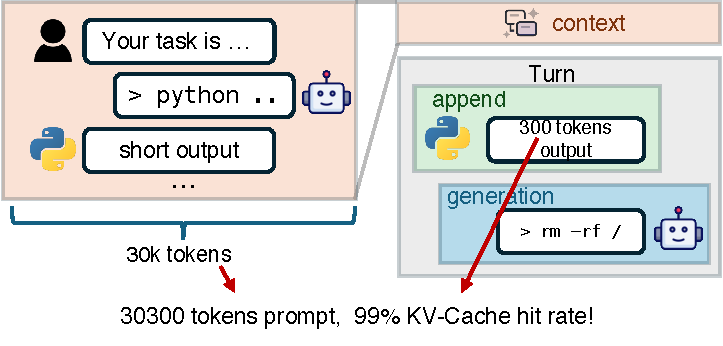
\includegraphics[width=\linewidth]{figures/workload}
  \vspace{-0.3in}
  \caption{\normalfont Agent trajectory example.}
  % \vspace{-0.2in}
  \label{fig:workload}
\end{figure}

LLMs increasingly power \emph{agentic} applications that perform multi-turn reasoning and interact with an environment (via e.g., terminal commands, code execution, or asking for human feedback) over long sessions. 
As shown in \autoref{fig:workload}, in a typical \emph{turn}, the model receives a prompt composed by the previous \emph{context} plus some newly \emph{appended tokens} (often tool output or user input) and \emph{generates} the next action or response. A single agent run is a \emph{trajectory} of dozens or even hundreds of turns: the context grows turn-by-turn and can reach up to one million tokens \cite{claudeopus46, googlegemini3pro}. 
Because most of the context, typically >95\% tokens in our traces, is reused across rounds, the vast majority of tokens in each round can hit the KV-Cache; only the newly appended context needs prefill computation. Due to the extreme length of agent trajectories, DRAM and HBM-based KV-Cache storage like Mooncake \cite{FAST25:Mooncake} can only store a small proportion of KV-Caches, necessitating the use of larger yet cheaper external SSD-based KV-Cache storage \cite{3FS}.

The agentic LLM inference workload is also prevalent in agent LLM training, which often adopts \emph{reinforcement learning} (RL) approaches. In a typical RL training loop, the agent LLM first undergoes a \emph{rollout} phase, where it is prompted to generate a large number of multi-step agent trajectories. These trajectories are then scored by a separate reward model. Finally, the LLM parameters are updated to increase the likelihood of high-scoring outputs and reduce the likelihood of low-scoring ones. During the rollout phase, substantial data (like reward model and optimizer states) is offloaded to host DRAM, further constraining the available DRAM for KV-Cache. This reinforces the need for external, high-capacity KV-Cache storage that can accommodate long agentic rollout contexts efficiently.

\subsection{Modern AI Data Center Architecture}

Modern AI data centers are purpose-built logical supercomputers engineered to handle large-scale generative AI training and inference workloads. For example, in a standard NVIDIA DGX SuperPOD \cite{nvidia2023superpod}, each node is equipped with 8 Hopper GPUs interconnected via high-speed NVLink. Each GPU is paired with a dedicated 400 Gbps compute NIC (\emph{CNIC}, also known as east-west NIC), which maximizes inter-node communication bandwidth. Independent of the compute fabric, each node also features a storage NIC (\emph{SNIC}, also known as south-north NIC) up to 400 Gbps, providing fast access to datasets, model checkpoints, and on-disk KV cache.

A fundamental principle of this architecture is that the compute network and the storage network are isolated from each other \cite{zhao2025insights}. This separation is essential to maximize both storage and application performance. By isolating high-intensity east-west compute traffic between GPUs from storage traffic, the architecture prevents interference between them, and drastically reduces compute communication latency. This design also ensures that the inter-GPU communication remains highly reliable and predictable even when performing data-intensive tasks such as reading large datasets or writing multi-terabyte model checkpoints.